\chapter{Construcción Secuencial sujeta a $RG$}
\label{champ:BSGR}
\bigskip
\barra
\bigskip

%En este capítulo se describen dos algoritmos para la creación de redes porosas sujetas a restricciones geométricas. En ambos algoritmos la generación de sitios y enlaces se basa en las distribuciones $F_S(R_S)$ y $F_B(R_B)$. La primera propuesta esta basada puramente en el Método de Monte Carlo para la generación de redes porosas que cumplan con las restricciones geométricas. El segundo algoritmo propuesto tanto los sitios como los enlaces son generados y ordenados de forma descendente en dos listas respectivamente, de igual forma existe un proceso de sembrado de semillas para la generación de clusters dicho proceso se basa en la asignación de sitios de mayor tamaño primero, los sitos asignados a la red porosa no tienen ningún enlace conectado a diferencia del algoritmo secuencial de NoMISS donde los sitios semilla debían tener sus seis enlaces conectados. Después del proceso de sembrado comienza la asignación de enlaces donde en el primer algoritmo la asignación es puramente aleatoria, el segundo algoritmo se intenta conectar cada enlace con el sitio mas grande posible. Detallamos cada algoritmo en las siguientes secciones.


En este capítulo se describen dos algoritmos para la creación de redes porosas sujetas a restricciones geométricas. En ambos algoritmos la generación de sitios y enlaces se basa en las distribuciones $F_S(R_S)$ y $F_B(R_B)$. Ambos algoritmos propuestos se pueden separar en dos grandes fases: inicalizaci\'on de la red porosa con sitios y enlaces y la generación de una red porosa v\'alida. Cabe señalar que una red porosa v\'alida es aquella que se encuentra libre de violaciones a las $RG$. En la primera fase el primer algoritmo inserta de forma aleatoria sitios y enlaces hasta cubrir toda la red, mientras tanto el segundo algoritmo sigue el método de sembrado del algoritmo secuencial NoMISS. con la diferencia de que los sitios que conforman a los clusters no tienen enlaces asignados inmediatamente después del sembrado el algoritmo comienza a asignar enlaces a los sitios siguiendo la regla de intentar conectar siempre a cada sitio los enlaces de mayor tamaño posible. Después de la fase de inicalizaci\'on ambos algoritmos pueden tener violaciones a las $RG$ por lo que la segunda fase se basa en la eliminaci\'on de las violaciones a las $RG$ utilizado el Método de Monte Carlo. A continuación se describe a detalle cada algoritmo.

\section{Solución Básica Aleatoria}
\label{sec:smcrg}
En este algoritmo tiene por objetivo inicializar la red porosa con sitios y enlaces de forma aleatoria en dos pasos, en el primer paso se generan e insertan en la red porosa $L^3$ sitios en base a la distribución $F_S(R_S)$, conforme se van generando los sitios estos se insertan en la red porosa. El segundo paso consiste en conectar tres enlaces a cada sitio de la red porosa, cada enlace es generado en base a la distribución $F_B(R_B)$ y al final tendremos $3 \cdot L^3$ enlaces dentro de la red porosa.\\
%Después de la inicailizaci\'on se aplica el Método de Monte Carlo sobre la red hasta eliminar todas las violaciones a las $RG$ tal y como se describe mas adelante en la sección \ref{sec:svalid}.\\

Cabe destacar que aun cuando se le asignaron solo tres enlaces a cada sitio, la conectividad de estos sigue siendo igual a seis debido a que los otros tres enlaces los comparte con sus sitios vecinos siguiendo una topología tipo toro tal y como se muestra en la Figura \ref{fig:redinit} donde se puede apreciar que al sitio de color gris obscuro le comparten un enlace cada uno de sus sitios vecinos que están representados en color gris claro, a su vez el sito de color gris obscuro le comparte sus enlaces a los sitios que se encuentran en la posición frente-inferior-derecho, trasero-superior-derecho y frente-superior-izquierdo de la red porosa.


\begin{figure}[hbtp]
\centering
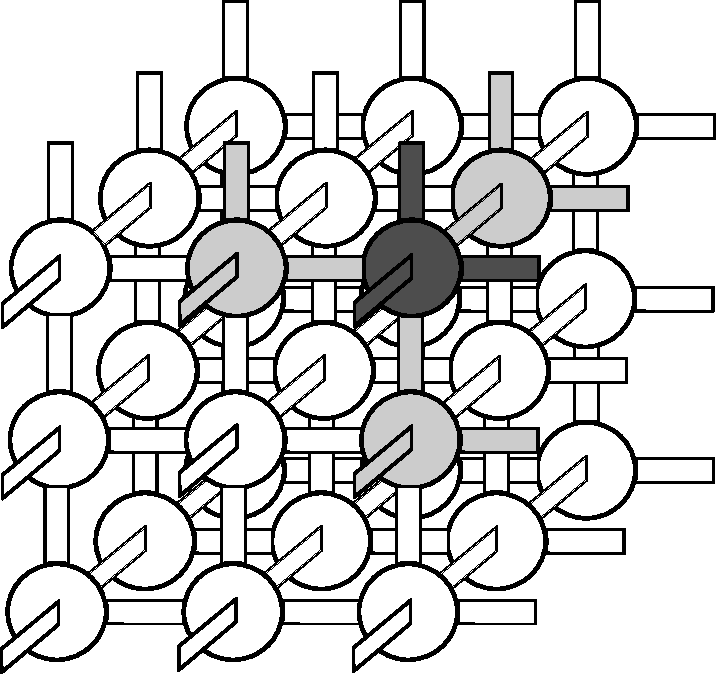
\includegraphics[width=2.8in]{img/red2.pdf}
\caption{Red porosa inicalizada con $L^3$ sitios y $3 \cdot L^3$ enlaces}
\label{fig:redinit}
\end{figure}

\section{Solución Híbrida}
\label{sec:hybrid}
El algoritmo que se presenta a continuación inicializa una red porosa con sitios y enlaces donde se intenta que la conexi\'on entre estos cumpla con las $RG$. La primera acción del algoritmo es crear dos listas de tamaños de poros ordenadas de forma descendente(en base al tamaño de los sitios o enlaces respectivamente) mediante un algoritmo de ordenamiento por inserción. La primera lista $L_S$ se compone de $L^3$ sitios mientras que la segunda $L_B$ contiene $3L^3$ enlaces. Subsecuentemente a la creaci\'on de  las listas se lleva acabo el proceso de sembrado y rellenado similar al aplicado en el algoritmo NoMISS descrito en la Sección \ref{subsubsec:nomiss} después del sembrado y rellenado sigue el proceso de asignación de enlaces a los sitios. A continuación se describe a detalle el algoritmo.

%En este algoritmo se propone una nuevo algoritmo para la construcción de redes porosas sujetas a $RG$ el cual a diferencia del algoritmo de la sección anterior que inicializa de forma aleatoria toda la red porosa por lo cual no se validan las $RG$, en algoritmo descrito en esta sección a cada sitio se intenta conectar con los enlace más grandes posibles y intentar que se cumplan con las $RG$, cabe destacar que es posible que una conexión no cumpla con las $RG$ para lo cual y de igual forma que en el algoritmo de la sección anterior aplicaremos el Método de Monte Carlo hasta eliminar las violaciones a las $RG$. En este algoritmo se intenta mejorar la isotropía a partir de la inicialización por lo cual se lleva acabo un proceso de sembrado y rellenado similar al aplicado en el algoritmo NoMISS descrito en la sección \ref{subsubsec:nomiss}. A continuación se describe de forma detalla los pasos que conforman el algoritmo. 

%\subsection{Generación de Sitios y Enlaces}
%\label{subsec:hybridgse}
%En este paso, se generan dos listas de tamaños de poros ordenadas de forma descendente(en base al tamaño de los sitios o enlaces respectivamente) mediante un algoritmo de ordenamiento por inserción. La primera lista $L_S$ se compone de $L^3$ sitios mientras que la segunda $L_B$ contiene $3L^3$ enlaces.

\subsection{Sembrado de Clusters}
\label{subsec:sseeding}
Durante todo el proceso de sembrado y rellenado de la red porosa cada vez que se toma un elemento de la lista $L_S$ se hace referencia a que se toma el primer elemento actual de $L_S$ siendo este el sitio actual más grande.\\

El proceso de sembrado de clusters se divide en dos pasos el primer paso consiste en tomar el primer sitio (semilla) de la lista $L_S$ e insertarlo en una posición aleatoria de la red porosa, el segundo paso consiste en tomar más elementos de $L_S$ y uno a uno insertarlos alrededor de la semilla actual hasta de crear un cluster de sitios de tamaño $ClusterSize$ el cual tendrá la forma de un cubo; este procedimiento se describe en las lineas 1-6 del Algoritmo \ref{alg:seedingalg}. En la Figura \ref{fig:cluster} se muestra de forma gráfica la creación de un cluster donde $ClusterSize=3$.\\

Cada vez que se inserta un elemento de $L_S$ en una posición aleatoria $(i,j,k)$ de la red, dicha posición se almacena en la lista $L_{SC}$ que se mantiene ordenada de forma descendente en base al tamaño de los sitios insertados. El procedimiento de inserción de semillas y la creación de un clusters de tamaño $ClusterSize$ se repite $p$ veces, donde $p$ es un número de clusters a insertar. En caso que durante la creación de los clusters exista un traslape entre ellos, el sembrado se omite en las regiones ya ocupadas(en las que existe traslape) y se continua el sembrado de los sitios en los espacios aun vacíos.\\

\begin{figure}[hbtp]
\centering
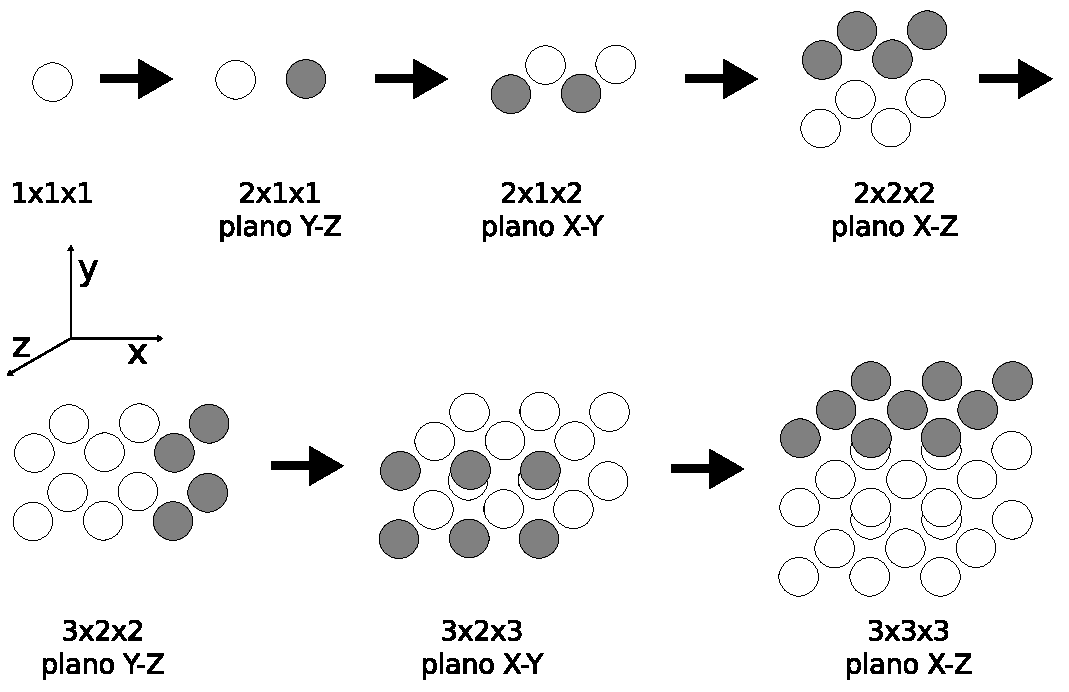
\includegraphics[width=5.0in]{img/cluster_es.pdf}
\caption{Sembrado de un cluster de tamaño 3x3x3}
\label{fig:cluster}
\end{figure}

En la Figura \ref{fig:cluster1} se muestra una red porosa después del proceso de siembra de $p$ clusters de tamaño $3x3x3$ cada uno, también se puede observar que en la red quedan espacios vacíos  los cuales serán rellenados de la siguiente forma: una vez completado el proceso de siembra de clusters, al primer cluster generado se le insertan alrededor suyo todos los sitios restantes de $L_S$(lineas 7-9 del Algoritmo \ref{alg:seedingalg}) siguiendo las mismas reglas de construcción de cluster anteriores, con al diferencia de que se establece $ClusterSize=L$ con lo cual se garantiza que se ocuparan todos los espacios vacíos de la red porosa.\\

\begin{figure}[h]
\centering
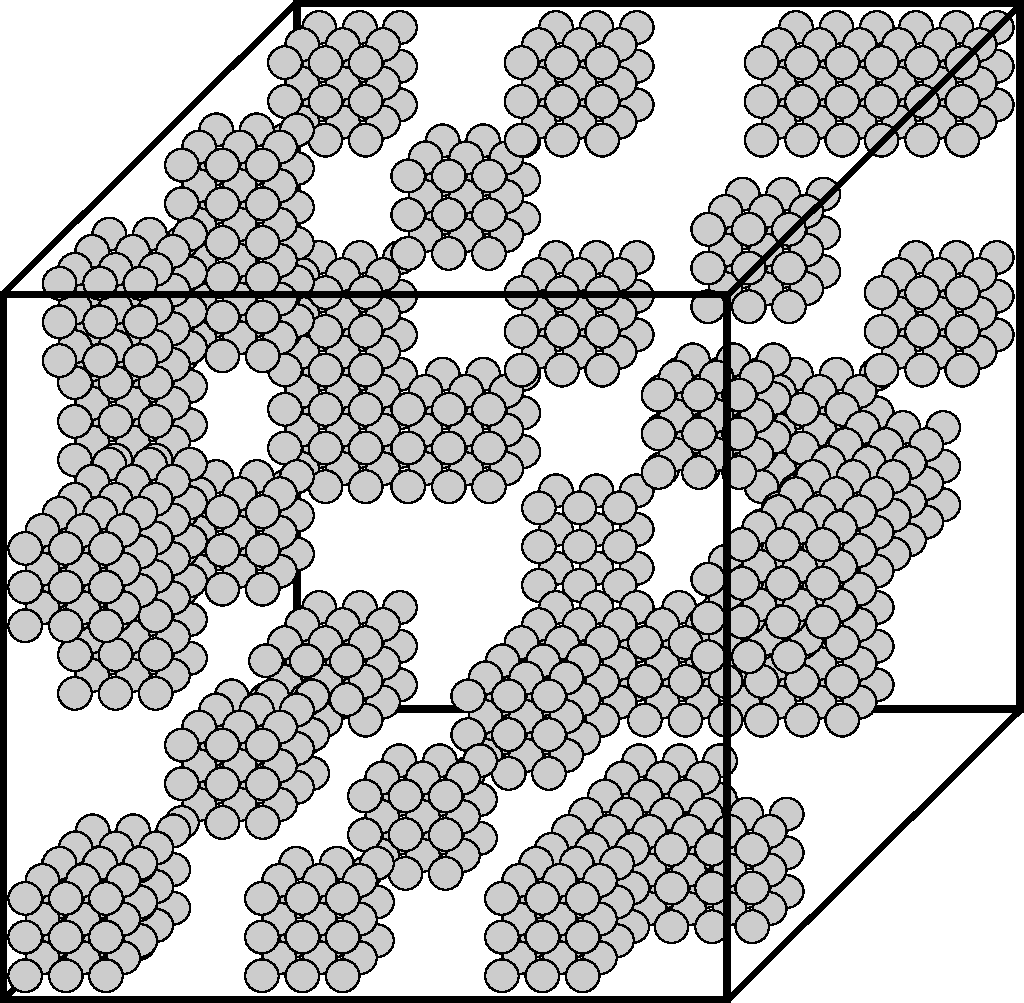
\includegraphics[width=3.0in]{img/cluster1.pdf}
\caption{Red Porosa después del proceso de siembra de clusters}
\label{fig:cluster1}
\end{figure}

\begin{algorithm}
\caption{Sembrado de clusters dentro de la red porosa($pnet$)}\label{alg:seedingalg}
\begin{algorithmic}[1]
\Require $L_S$, $L_{SC}$, $NClusters$, $ClusterSize$ 
\For{$m\gets 1$ \textbf{to} $NClusters$}
\State $pnet[i][j][k] \gets $ \Call{First}{$L_S$} {$//\;i,j,k$:posición aleatoria}
\For{$p\gets 1$ \textbf{to} $ClusterSize$}
\State \Call{InsertPCluster}{$pnet,i,j,k,\&L_S,\&L_{SC}$}
\EndFor
\EndFor
\While{\Call{Size}{$L_S$} $> 0$} {$//\;i,j,k$:La posición de la primera semilla}
	\State \Call{InsertPCluster}{$pnet,i,j,k,\&L_S,\&L_{SC}$}
\EndWhile
\end{algorithmic}
\end{algorithm}

Al final del proceso de siembra y rellenado, los sitios en su mayoría tienen a su alrededor sitios con tamaños similares con lo cual se tiene mayor oportunidad de encontrar soluciones válidas al conectar los sitios con los enlaces y que cumplan con las $RG$, esto se debe a que es mas sencillo encontrar un enlace para conectar dos sitios similares a encontrar un enlace que conecte dos sitios de tamaños distintos(o muy distintos). En contraste con la versiones de NoMISS descritas en el Capítulo \ref{champ:relatedwork}, en este algoritmo los sitios insertados durante el sembrado y rellenado no tienen aún enlaces asignados.\\

\subsection{Asignación de Enlaces}
\label{subsec:sbonds}
La asignación de enlaces se inicia con los sitos de más grandes hasta los sitios más pequeños. Para este fin, los elementos de la lista $L_{SC}$ son tomados uno a uno desde la primera posición de la lista. Como se menciono anteriormente, cada elemento de $L_{SC}$ contiene la posición en la cual se asigno cada sitio dentro de la red porosa, y el orden de los elementos es descendente en base al tamaño de los sitios, entonces el primer elemento de la lista siempre almacenara la posición dentro de la red del sitio más grande. Cuando un elemento es tomado de $L_{SC}$, se le intentan conectar $C$ enlaces al sitio en la posición correspondiente; los enlaces son tomados de la lista $L_B$, intentando usar los enlaces de mayor tamaño primero. Cada uno de los $C$ enlaces conectados a los sitios debería cumplir con el $PC$ y las $RG$. Solo en el caso que no exista un enlace en $L_B$ que cumpla con estas restricciones, para completar el contorno de enlaces se toma el enlace más grande de $L_B$ para ser conectado con el sitio actual, lo anterior permite la existencia de violaciones a las $RG$. En el Algoritmo \ref{alg:bondsalg} se muestra este comportamiento.\\

\begin{algorithm}
\caption{Asignación de enlaces}\label{alg:bondsalg}
\begin{algorithmic}[1]
\Require $L_B$, $L_{SC}$, $C=6$, $pnet$

\While{\Call{Size}{$L_{SC}$} $> 0$}
	\State $(i,j,k)\gets $\Call{First}{$L_{SC}$}
	\For{$p\gets 1$ \textbf{to} $C$} {$//\;C=6$ para una red cúbica}
		\State \Call{AssigneBondsRG}{$pnet,i,j,k,p,\&L_B$}
	\EndFor
\EndWhile
\end{algorithmic}
\end{algorithm}

\section{Generación de una red porosa válida}
\label{sec:svalid}


Una vez que la red porosa ha sido inicializada por completo ya sea con el algoritmo de la Solución Básica Aleatoria o con el de la Solución Híbrida con sitios y enlaces, la red porosa puede tener violaciones a las $RG$ esto se debe a que en la Solución Básica Aleatoria no se verifica el cumplimiento de las $RG$ al asignar un enlace a un sitio debido a que es un método completamente aleatorio, por el contrario la Solución Híbrida intenta conectar cada enlace con el sitio mas grandes posible donde la conexión entre sitio y enlace cumplan con las $RG$ sin embargo existen casos en los cuales no es posible que se cumplan las $RG$ y por consiguiente la conexión provoca violaciones a las $RG$. Cabe destacar que el número de violaciones a las $RG$ esta directamente relacionado con el valor del traslape($\Omega$).\\

%Una vez que la red porosa ha sido inicializada por completo con los sitios y enlaces ya sea con el algoritmo Solución Básica Aleatoria o con la Solución Híbrida la red porosas puede tener violaciones a las $RG$ esto se debe a que en el algoritmo Solución Básica Aleatoria no se verifica el cumplimiento de las $RG$ en la asignación de enlaces ya que es un método completamente aleatorio, por el contrario el algoritmo Solución Híbrida durante la asignación de enlaces este intenta conectar los enlaces de tal forma que cumplan con las $RG$ haciendo que los enlaces más grandes se conecten con los sitios más grandes sin embargo existen casos en los cuales no es posible realizar esta acción y por consiguiente pueden existir violaciones a las $RG$. Cabe destacar que el número de violaciones a las $RG$ esta directamente relacionado con el traslape($\Omega$).\\


Para eliminar las violaciones al $PC$ y $RG$ se utilizo en método el Método de Monte Carlo tal y como lo hace el algoritmo secuencial BiaSED descrito en la Sección \ref{subsubsec:biased}, entonces se aplica una serie de Pasos de Monte Carlo($MCs$) a la redes porosas generadas por los algoritmos descritos en las secciones \ref{sec:smcrg} y \ref{sec:hybrid} para eliminar por completo las violaciones tanto al $PC$ como a las $RG$.\\

En nuestro enfoque los intercambios de sitos o enlaces durante los pasos de Monte Carlo se deben cumplir tanto el $PC$ como las $RG$, en caso contrario el intercambio es rechazado, el algoritmo para la generación de una red porosa válida termina cuando todos los poros en la red cumplen tanto con el $PC$ como con las $RG$, como se muestra en el Algoritmo \ref{alg:validnet}.\\

\begin{algorithm}
\caption{Esquema de genración de una red porosa válida}\label{alg:validnet}
\begin{algorithmic}[1]
\Require $pnet$
\While{\Call{GRviolations}{$pnet$} $> 0$}
	\State \Call{PoreExchange}{$pnet$}
	\If{\Call{NonValidExchange}{pnet}}
		\State \Call{RejectExchange}{$pnet$}
	\EndIf
\EndWhile
\end{algorithmic}
\end{algorithm}

En las Figuras \ref{fig:mcs} y \ref{fig:mcsb} se muestra un ejemplo del intercambio válido de entre dos sitios y entre dos enlaces respectivamente, en Figuras \ref{fig:mcsc} y \ref{fig:mcsbc} se muestra un ejemplo de intercambio inválido de entre dos sitios y entre dos enlaces respectivamente. El tiempo que lleva el proceso de eliminación de violaciones al $PC$ y $RG$ varia dependiendo del traslape($\Omega$) entre las distribuciones utilizadas para generar a los sitios como a los enlaces de la red porosa y si este mismo es muy grande puede que el algoritmo \ref{alg:validnet} no termine.


\section{Mejoramiento de la isotropía}
\label{sec:isotropy}
Para que una red porosa válida sea lo más cercana a la realidad se requiere tanto del cumplimiento de las restricciones geométricas así como tener una buena isotropía es decir que los distintos tamaños de los poros estén lo mejor distribuidos en la red para lo cual después de generar una red porosa válida se aplican una número extra de $MCs$ siguiendo las mismas reglas utilizadas en la sección anterior, cabe destacar que el número extra de $MCs$ necesarios para mejorar la isotropía depende directamente del traslape($\Omega$) entre sitios y enlaces.


\begin{figure}[hbtp]
\centering
\begin{tabular}{cc}
\subfloat[Selección de los sitios a intercambiar]{
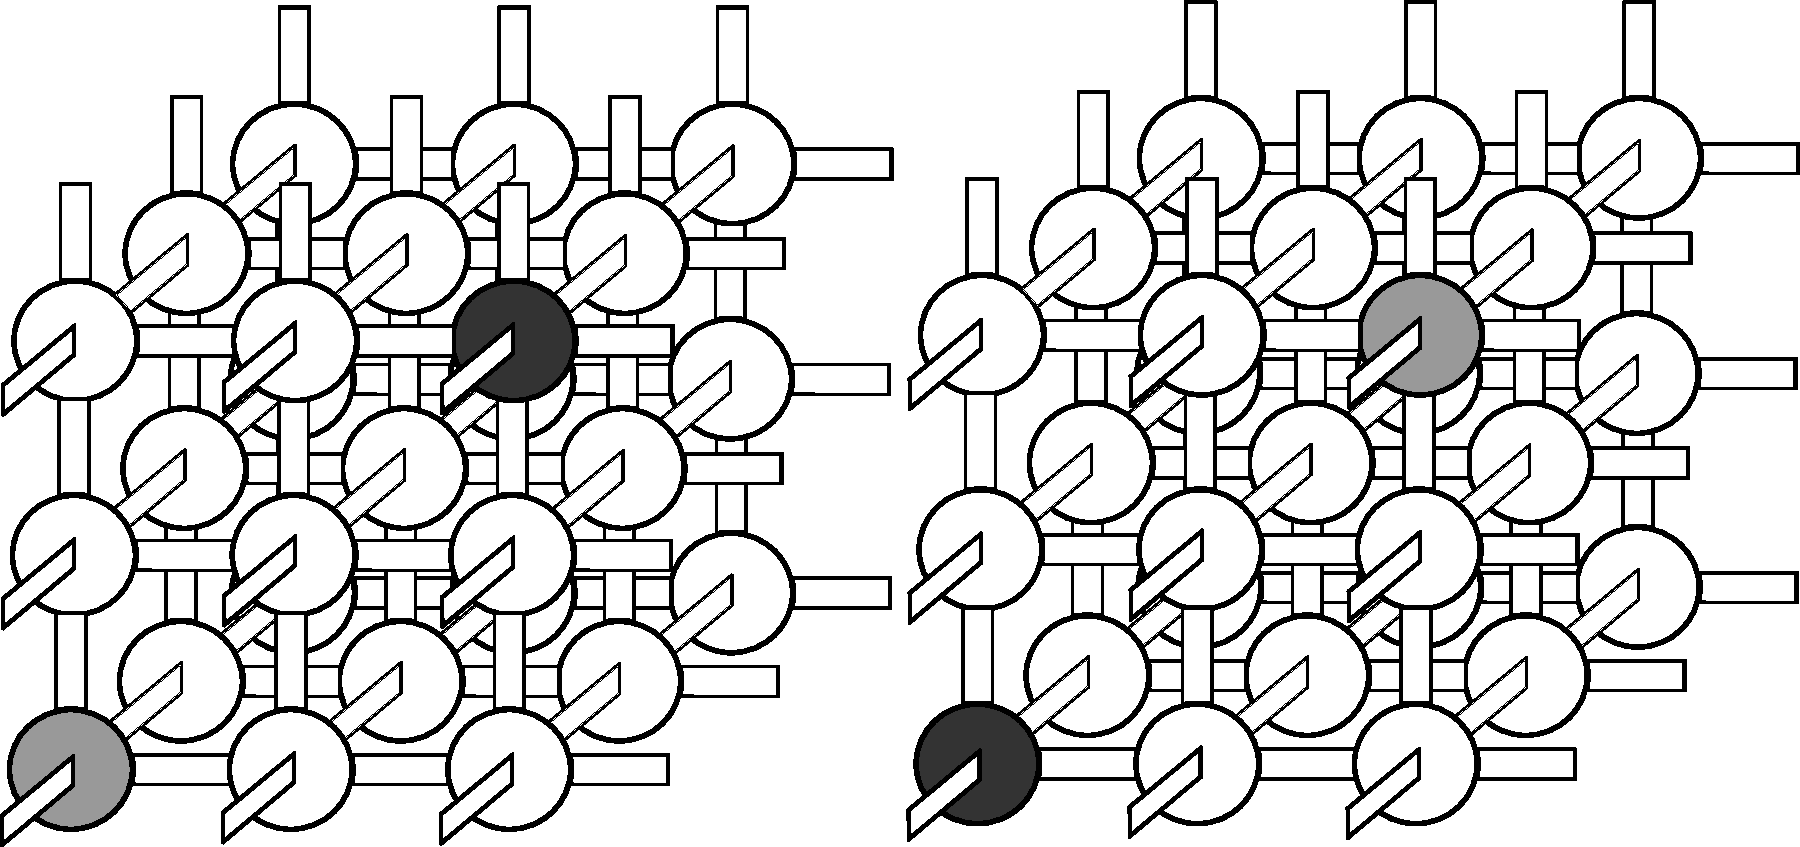
\includegraphics[width=2.5in, viewport=0 0 430 420,clip]{img/biased.pdf}
\label{fig:msc1}}
& \subfloat[Intercambio de sitios]{
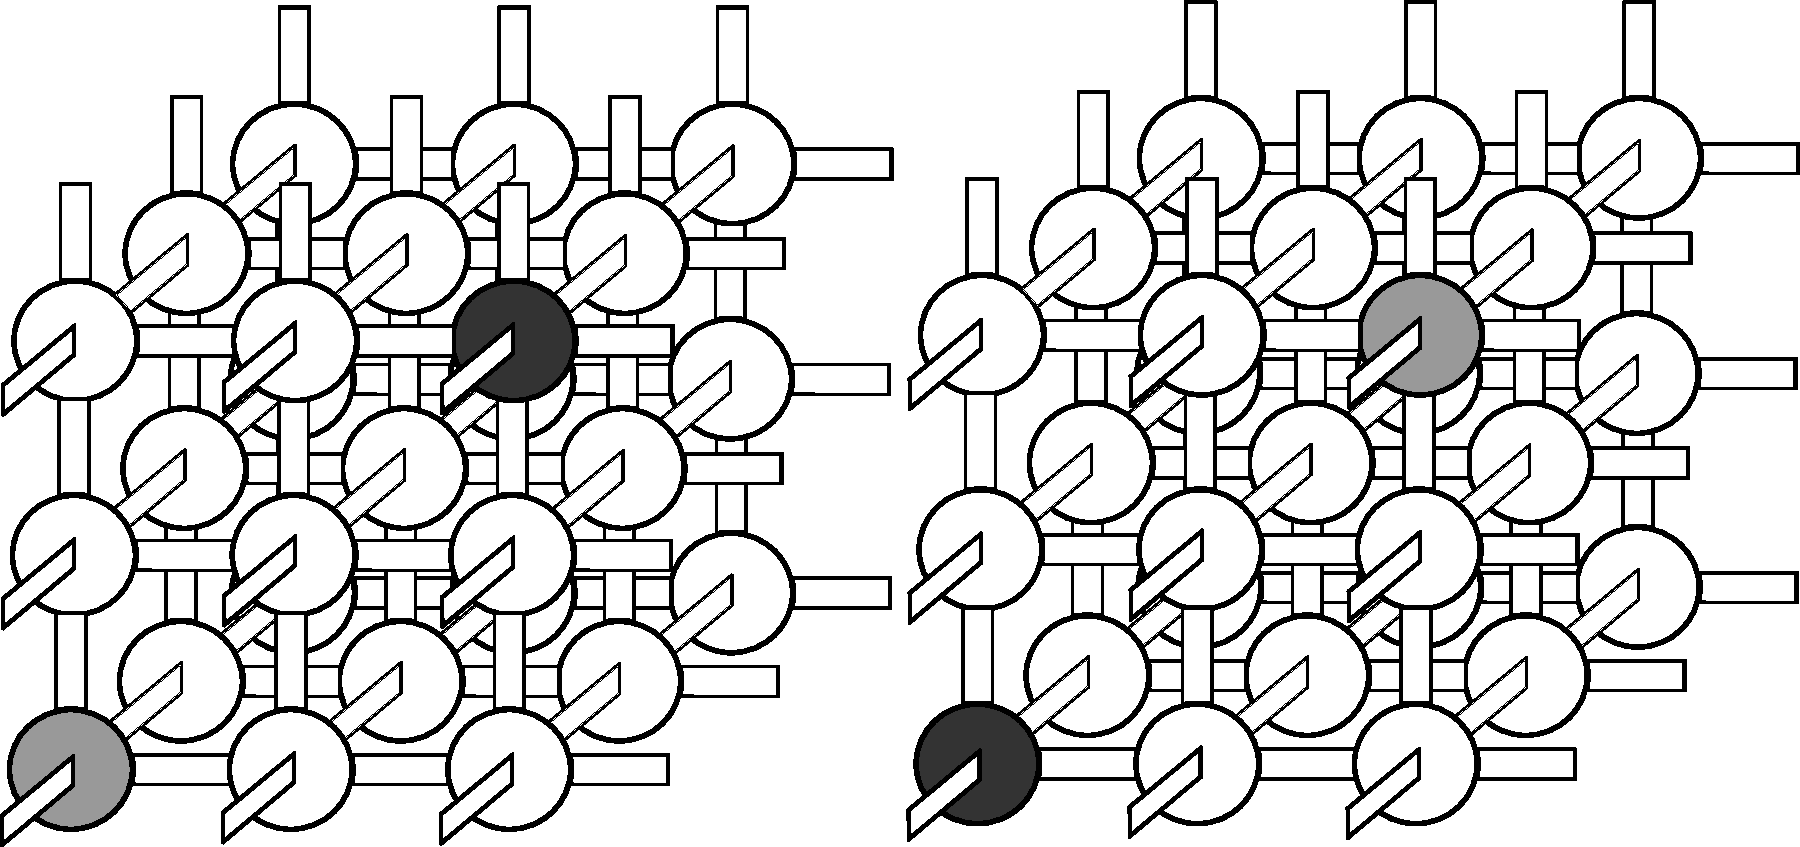
\includegraphics[width=2.5in, viewport=435 0 870 420,clip]{img/biased.pdf}
\label{fig:msc2}}
\end{tabular}
\caption{Ejemplo de un intercambio válido de dos sitios (a) selección y (b) intercambio}
\label{fig:mcs}
\end{figure}

\begin{figure}[hbtp]
\centering
\begin{tabular}{cc}
\subfloat[Selección de los enlaces a intercambiar]{
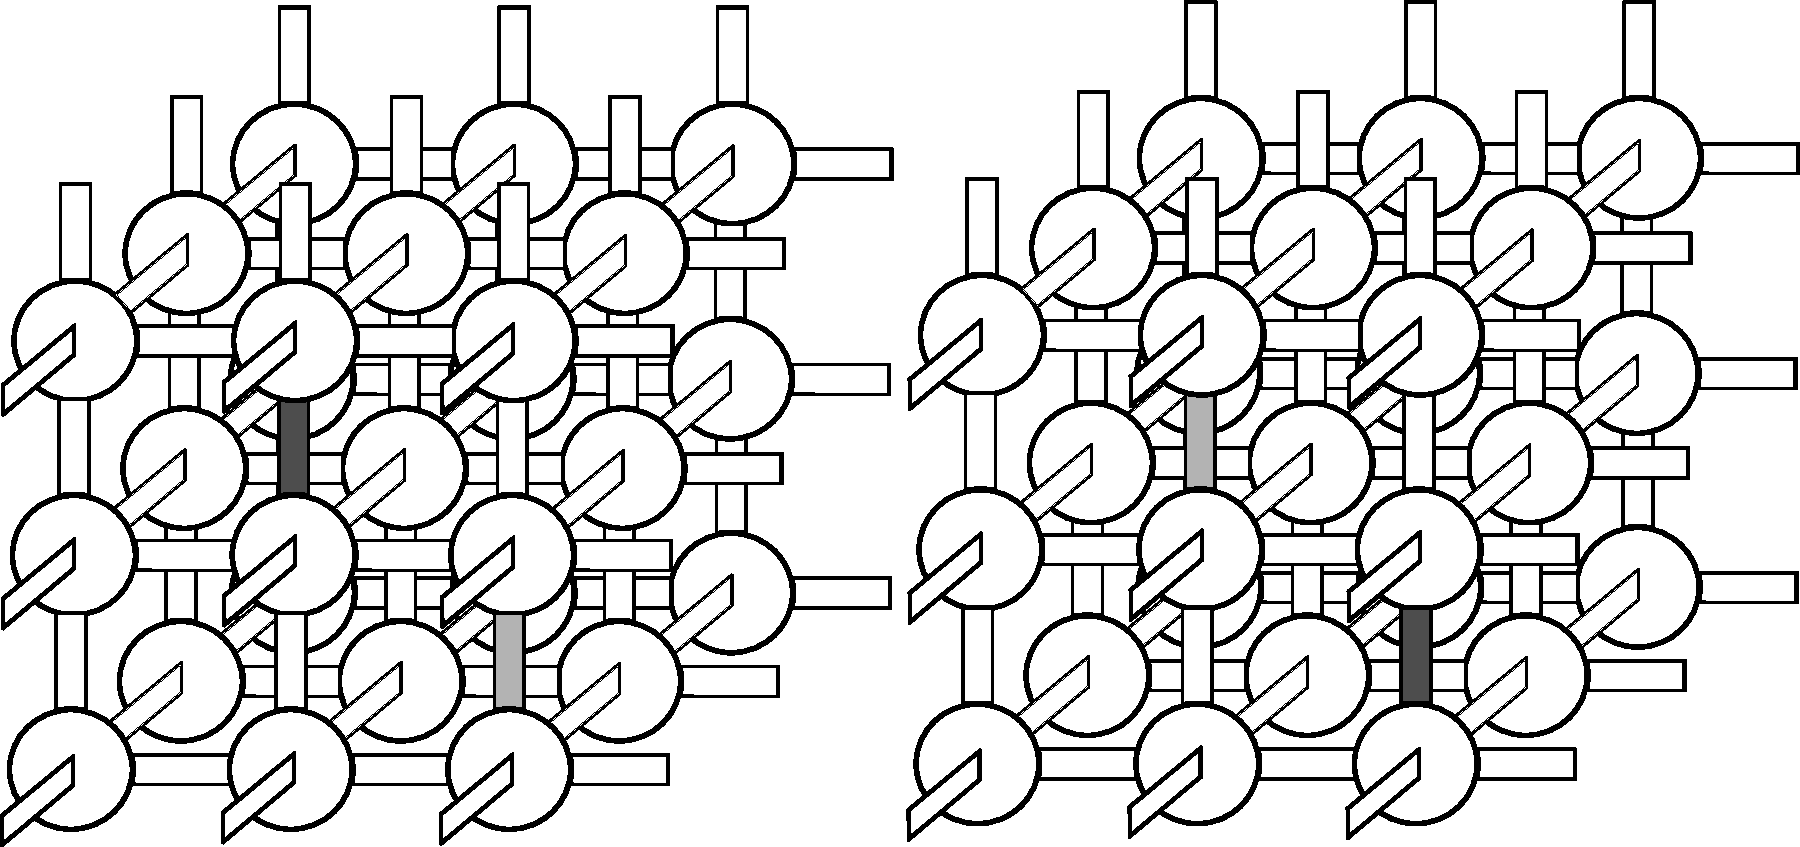
\includegraphics[width=2.5in, viewport=0 0 430 420,clip]{img/mcs.pdf}
\label{fig:mscb1}}
& \subfloat[Intercambio de sitios]{
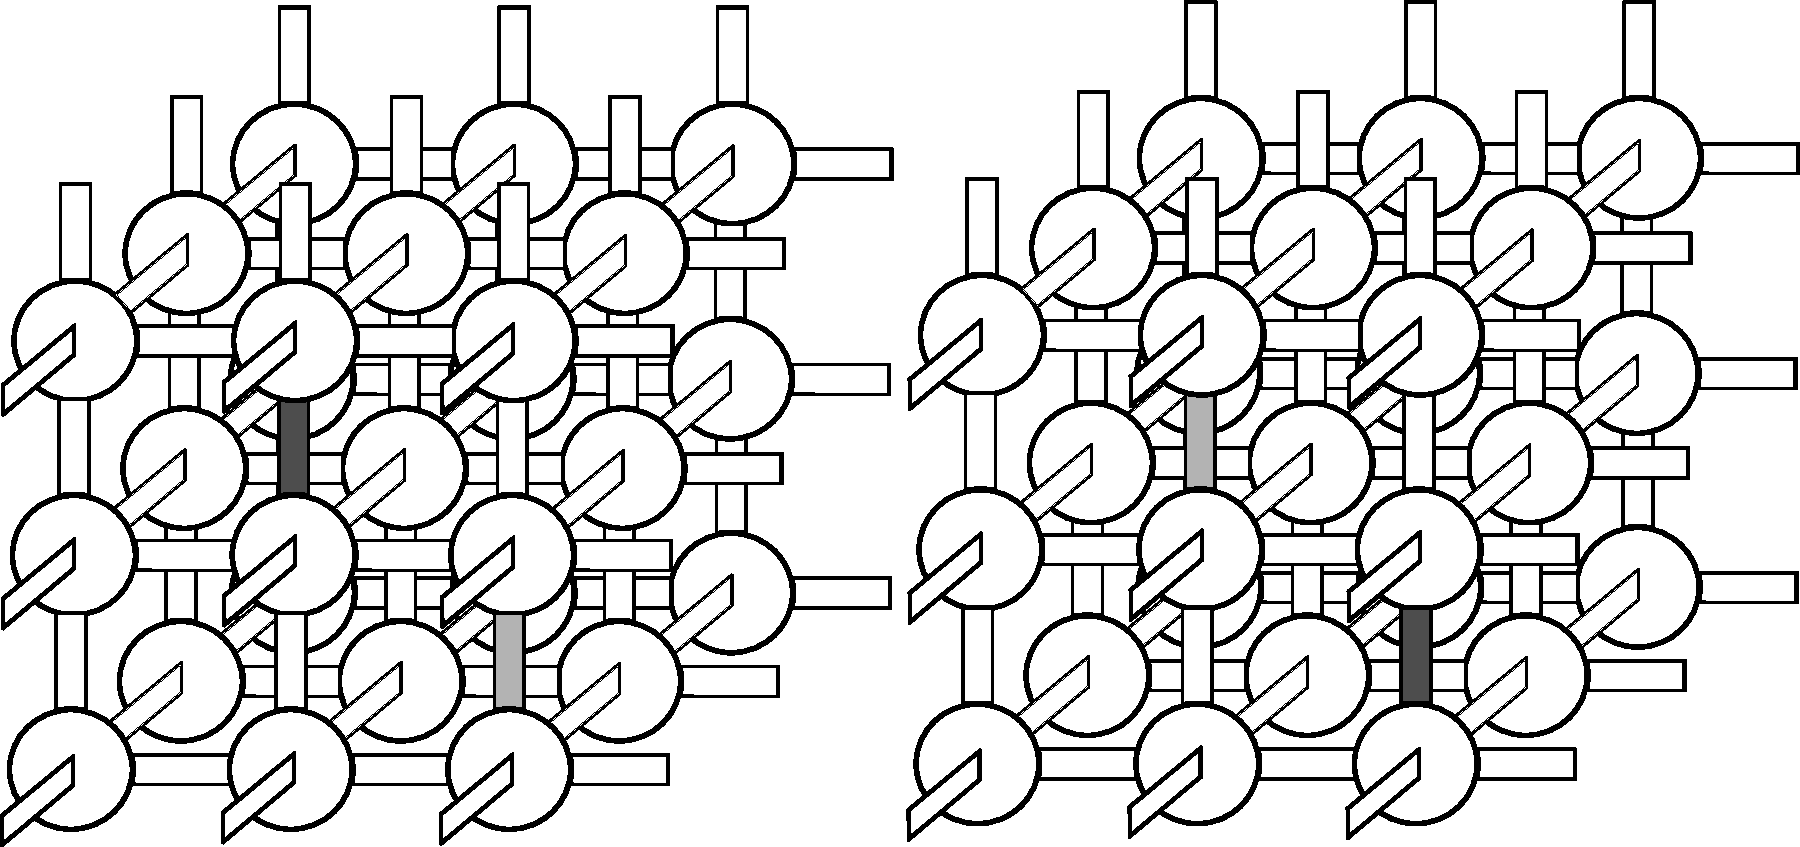
\includegraphics[width=2.5in, viewport=435 0 870 420,clip]{img/mcs.pdf}
\label{fig:mscb2}}
\end{tabular}
\caption{Ejemplo de un intercambio válido de dos enlaces (a) selección y (b) intercambio}
\label{fig:mcsb}
\end{figure}

\begin{figure}[hbtp]
\centering
\begin{tabular}{cc}
\subfloat[Selección de los sitios a intercambiar]{
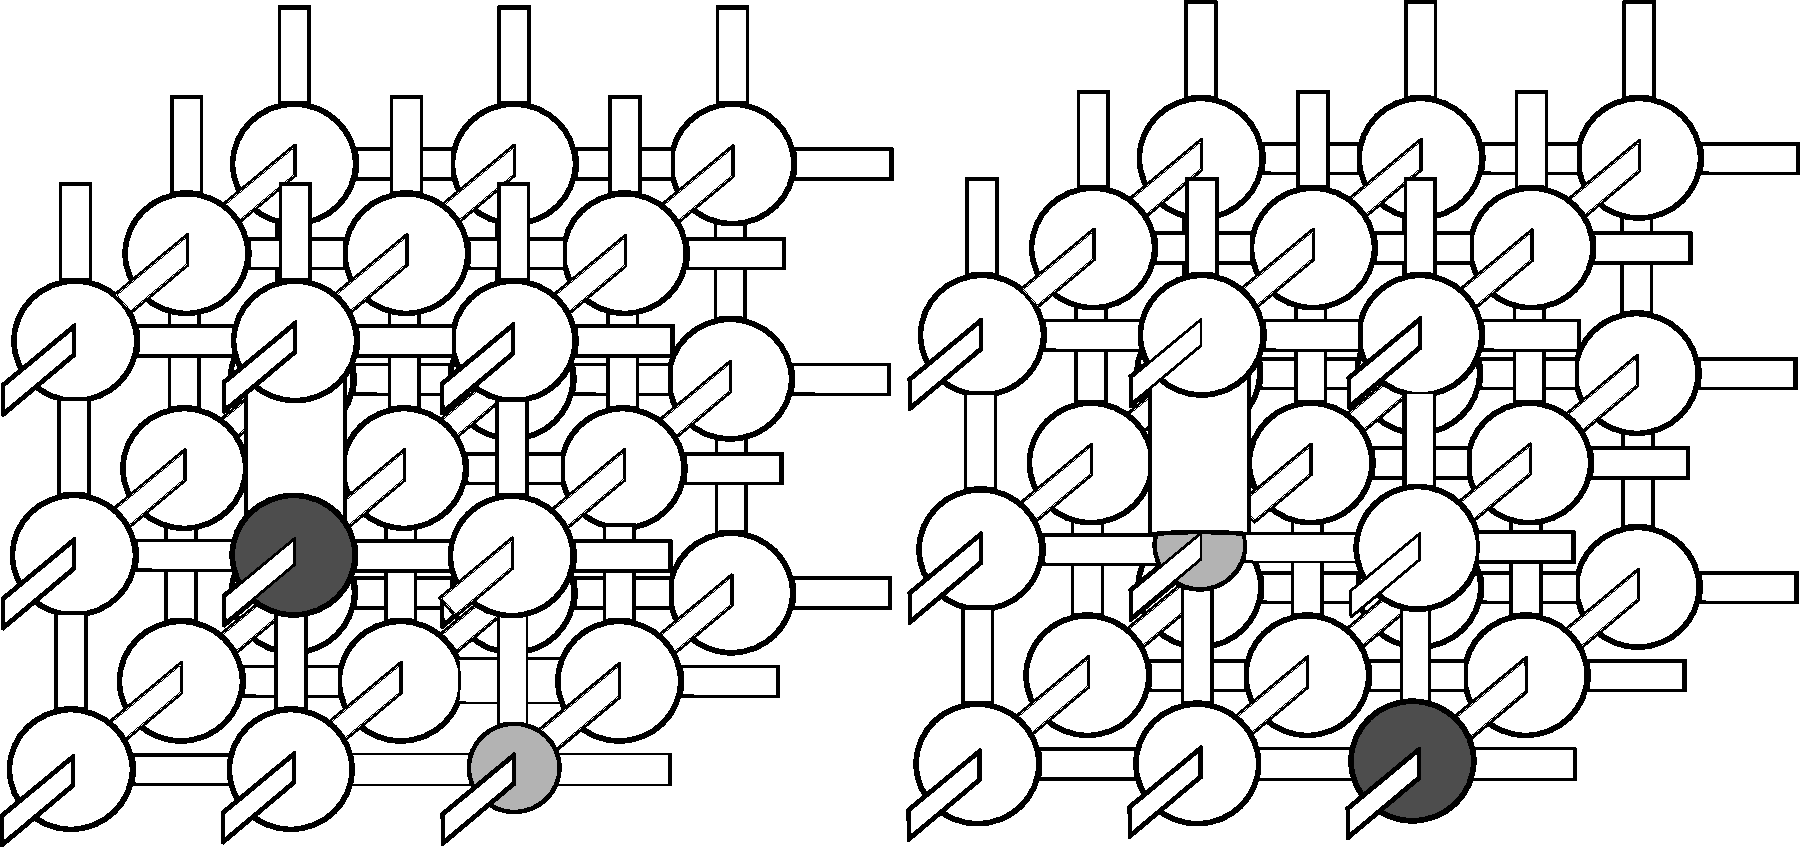
\includegraphics[width=2.5in, viewport=0 0 430 420,clip]{img/mcsc2.pdf}
\label{fig:msc3}}
& \subfloat[Intercambio de sitios]{
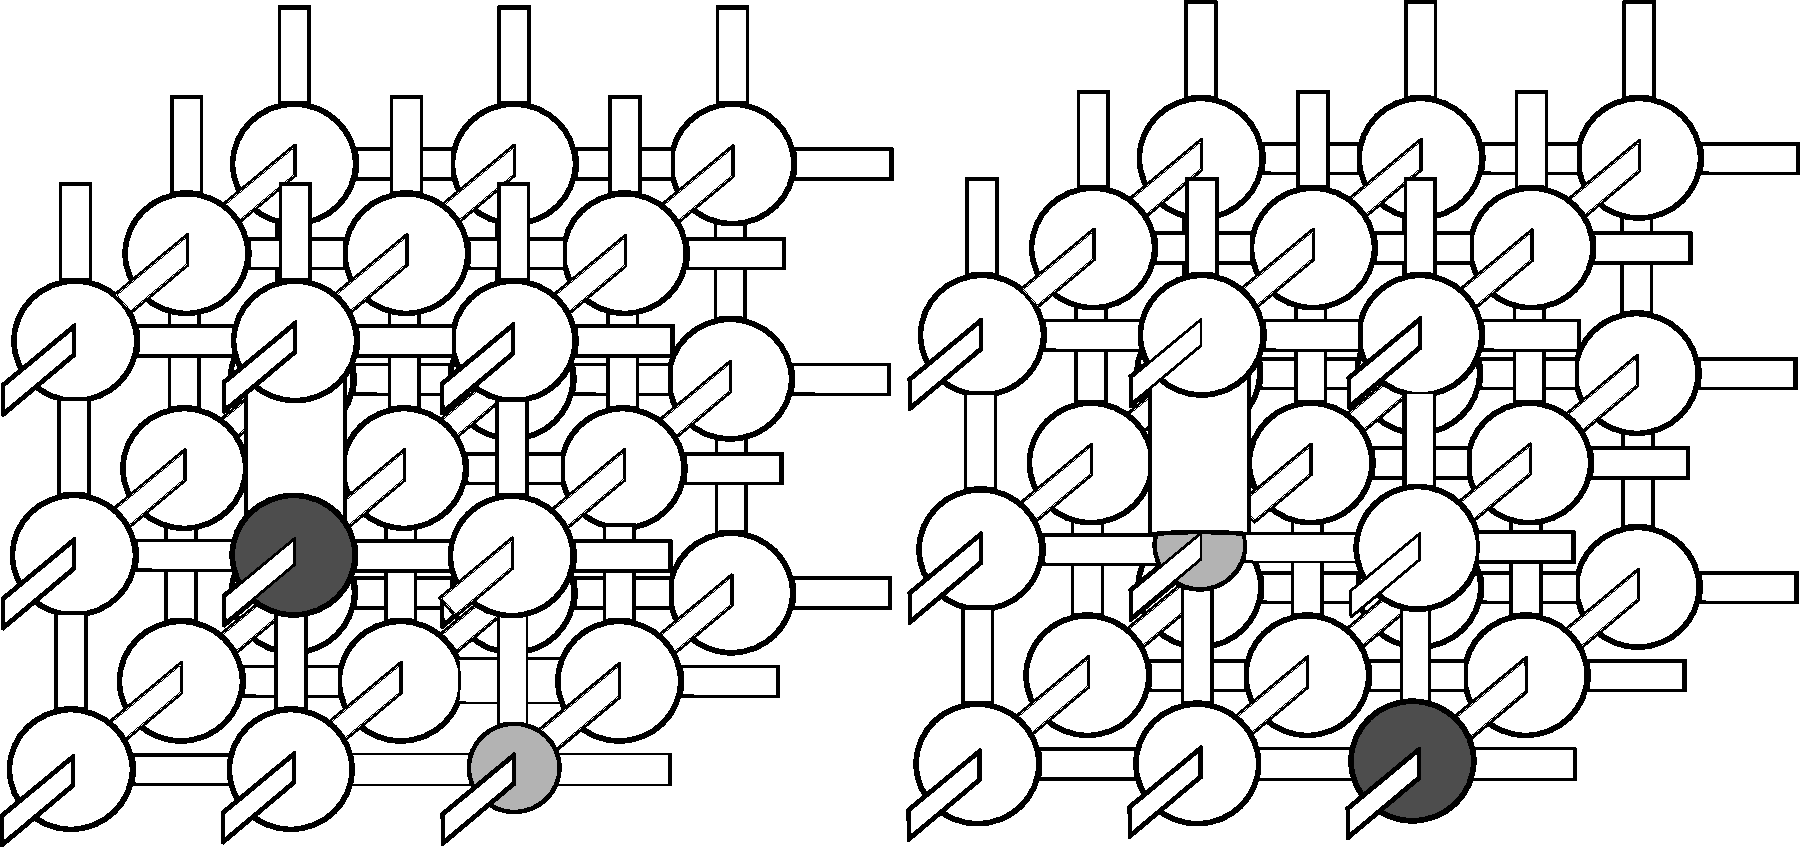
\includegraphics[width=2.5in, viewport=435 0 870 420,clip]{img/mcsc2.pdf}
\label{fig:msc4}}
\end{tabular}
\caption{Ejemplo de un intercambio inválido de dos sitios (a) selección y (b) intercambio}
\label{fig:mcsc}
\end{figure}

\begin{figure}[hbtp]
\centering
\begin{tabular}{cc}
\subfloat[Selección de los enlaces a intercambiar]{
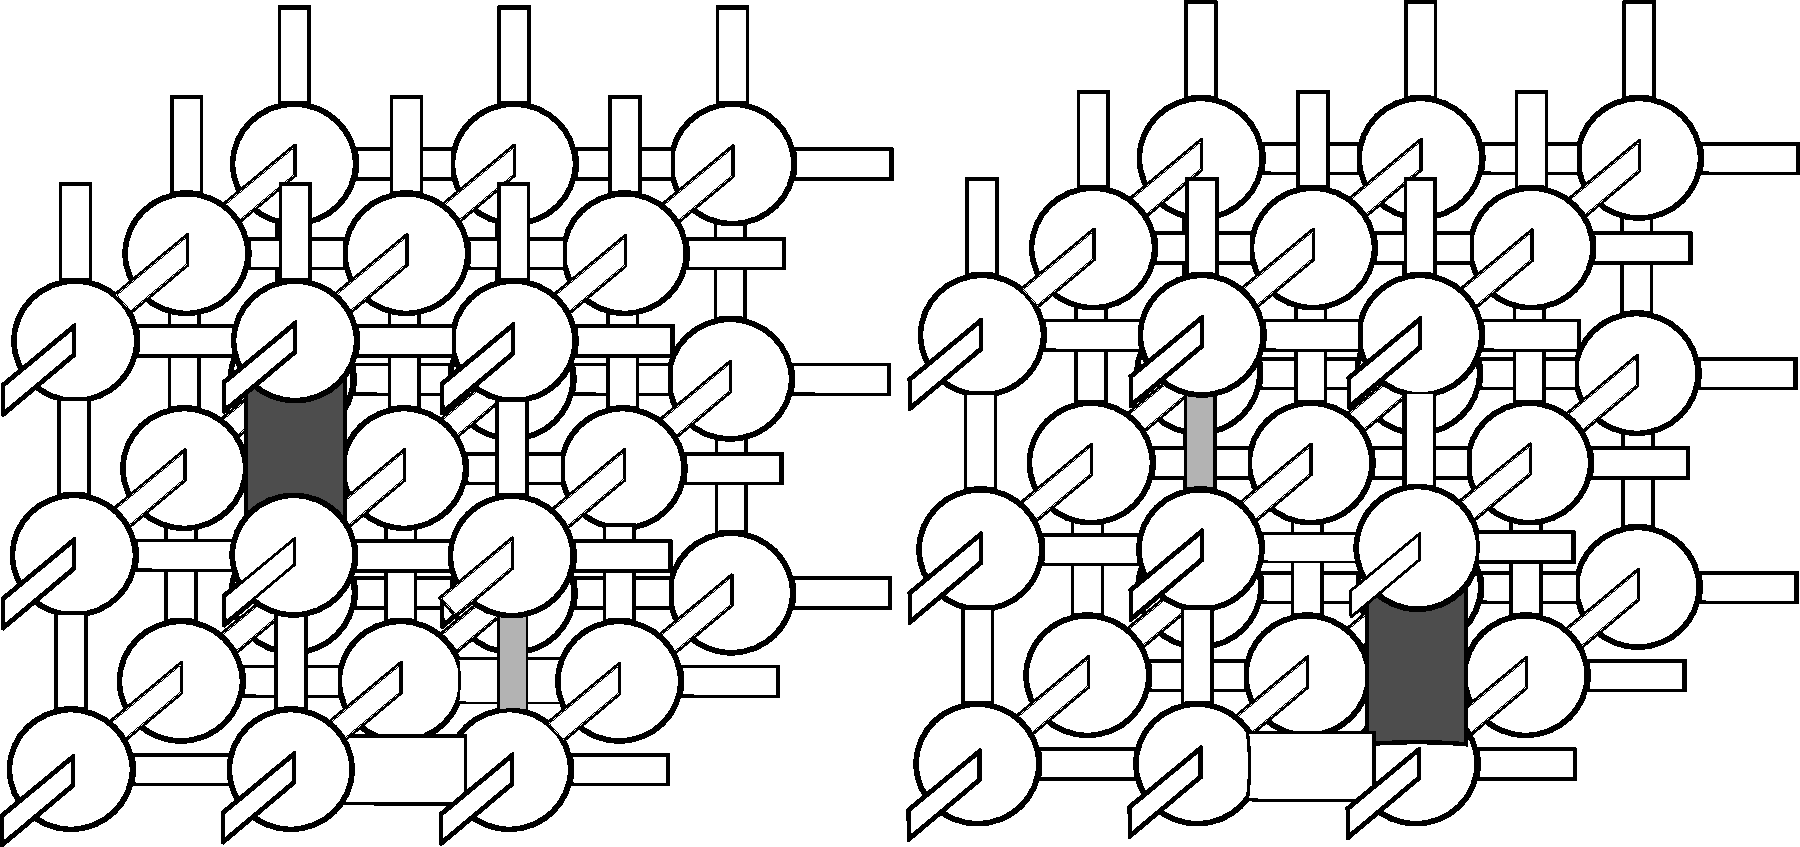
\includegraphics[width=2.5in, viewport=0 0 430 420,clip]{img/mcsc.pdf}
\label{fig:mscb3}}
& \subfloat[Intercambio de enlaces]{
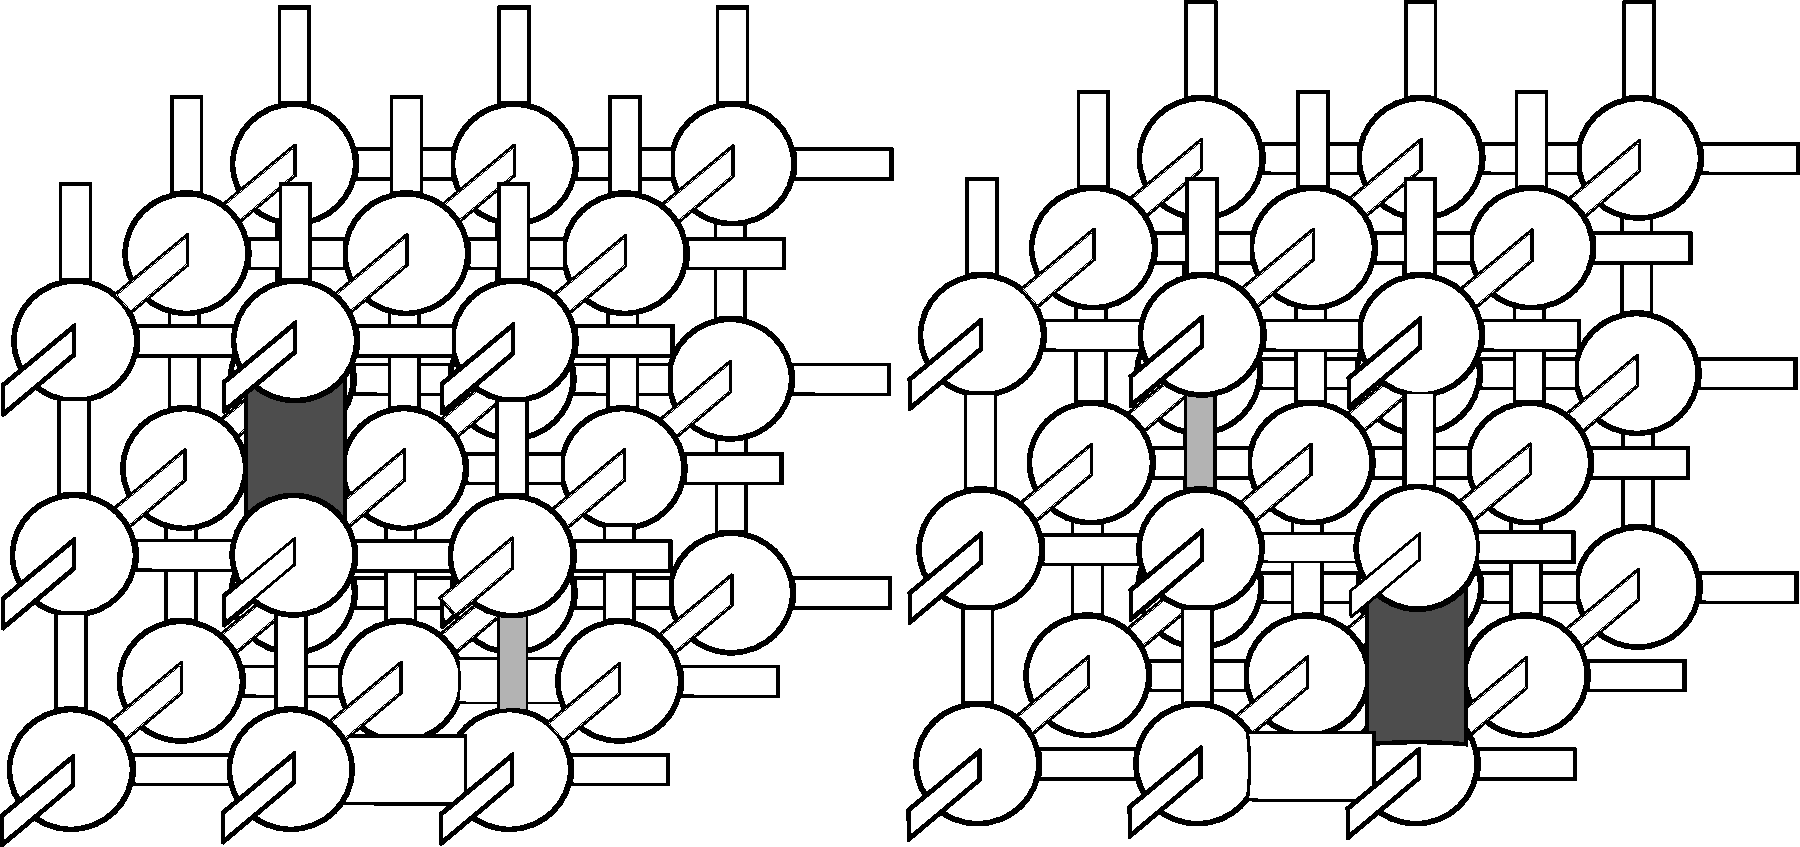
\includegraphics[width=2.5in, viewport=435 0 870 420,clip]{img/mcsc.pdf}
\label{fig:mscb4}}
\end{tabular}
\caption{Ejemplo de un intercambio inválido de dos enlaces (a) selección y (b) intercambio}
\label{fig:mcsbc}
\end{figure}

